\chapter{Machine learning algorithms comparison} \label{chap:methods}

%essayer d'autres noyaux pour SVM
%roc pour tous les scenariaux
%concatenate all datasets

Before going further and analysing neural networks, we will take a deeper look at classical machine learning algorithms, in particular Random Forest and Support Vector Machine (SVM) in the context of anomaly detection in the CPS presented in chapter \ref{chap:intro}. However this was done before in \cite{borges_hink_machine_2014-1} using the black-box model only. In their approach they used Weka \cite{witten_appendix_2017} in order to find the most performant algorithm among 7 they have chosen (OneR, NNge, Random Forest, Naïve Bayes, SVM, JRipper, Adaboost). Weka is an open source machine learning software. One of its advantages is a graphical interface, that is easy to use. 

The following sections show an attempt to reproduce the the results provided in \cite{borges_hink_machine_2014-1}, first using Weka, then scikit-learn \cite{pedregosa_scikit-learn_2011} to model the machine learning algorithms. The choice of scikit-learn was based on its versatility and configurability, which will be an asset in further modifications of the used algorithms.

\section{Weka} \label{sec:weka_in_chap:methods}
The dataset provided with \cite{adhikari_power_2014}\footnote{In fact there is three datasets available, differing by classification scheme: multiclass, three-class and binary. However, we are interested here only by the three-class dataset.} is composed of 15 sub-datasets, each one containing approximatively 5000 samples of different classes (i.e. Normal behaviour, Natural fault and Attack). Exactly like in \cite{borges_hink_machine_2014-1} the dataset was divided into 90\% training data and 10\% testing data and a tenfold cross validation methodology was applied in the training process. This methodology consists in randomly dividing the given training dataset into ten subsets, from which 9 will be used for the training and one for the validation. This process is repeated 10 times and the results are combined.  

The whole training process was done using the graphical interface of Weka for 5 machine learning techniques with standard parameters and then the results were analysed by generating four major indicators: accuracy, precision, recall and f-measure, and they stand for:
\begin{itemize}
    \item accuracy: ratio of correct classifications over the total number of samples,
    \item precision:  ratio of correct classifications for a particular class over all classifications that indicated that class,
    \item recall: ratio of correct classifications for a particular class, over all samples corresponding for this class,
    \item f-measure: weighted average of precision and recall given by the equation: \\f-measure\nolinebreak${= 2 \times \frac{\mathrm{precision} \times \mathrm{recall}}{\mathrm{precision} + \mathrm{recall}}}$.
\end{itemize}
The obtained values of those indicators were illustrated on figures \ref{fig:weka_acc3}, \ref{fig:weka_prec}, \ref{fig:weka_recall} and \ref{fig:weka_f1}. 

\begin{figure}[H]
    \centering
    \begin{subfigure}[t]{0.5\textwidth}
        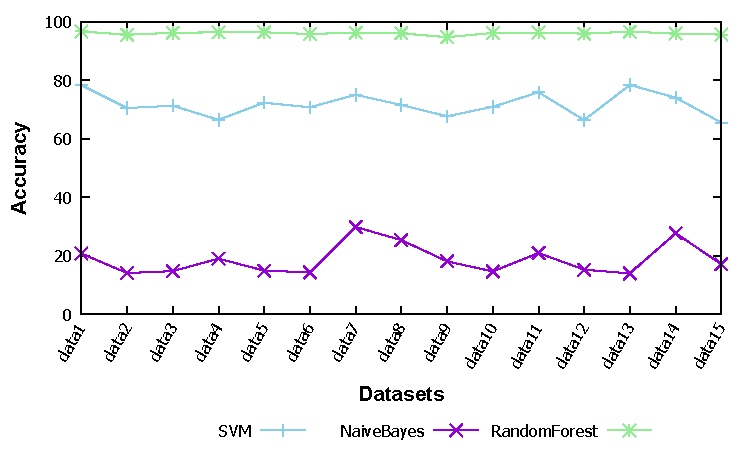
\includegraphics[width=\linewidth]{images/weka_accuracy3}
        \caption{Our attempt}
    \end{subfigure}%
    \begin{subfigure}[t]{0.5\textwidth}
        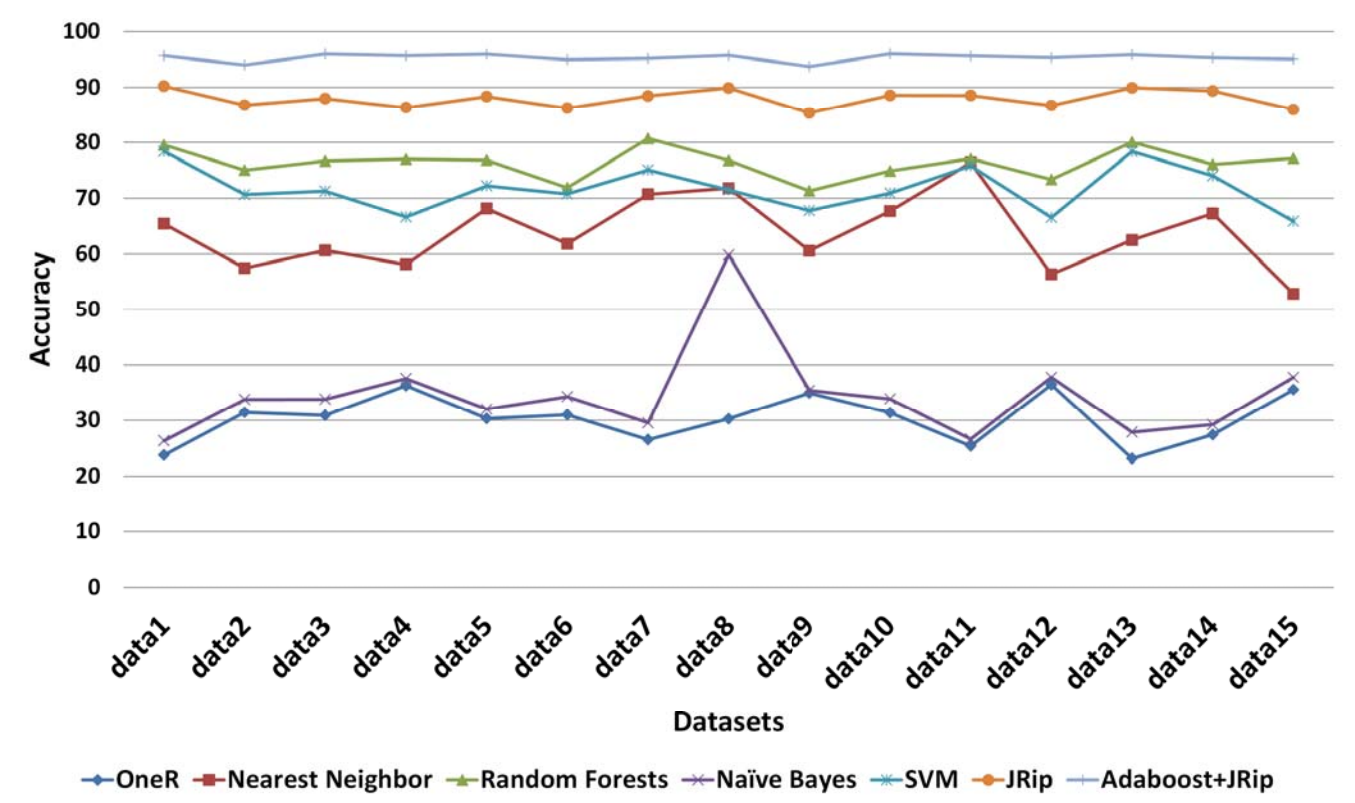
\includegraphics[width=\linewidth]{images/weka_accuracy3_cite.png}
        \caption{Original results \cite{borges_hink_machine_2014-1}}
    \end{subfigure}
    \caption{Accuracy for three-class datasets}
    \label{fig:weka_acc3}
\end{figure}

\begin{figure}[H]
    \centering
    \begin{subfigure}[t]{0.5\textwidth}
        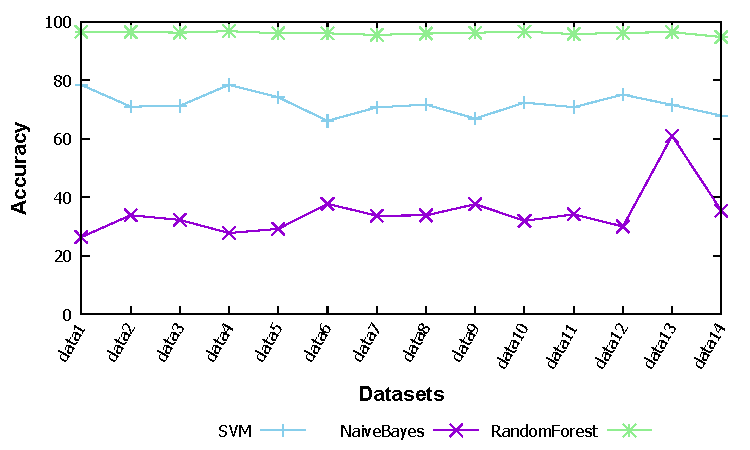
\includegraphics[width=\linewidth]{images/weka_accuracy2}
        \caption{Our attempt}
    \end{subfigure}%
    \begin{subfigure}[t]{0.5\textwidth}
        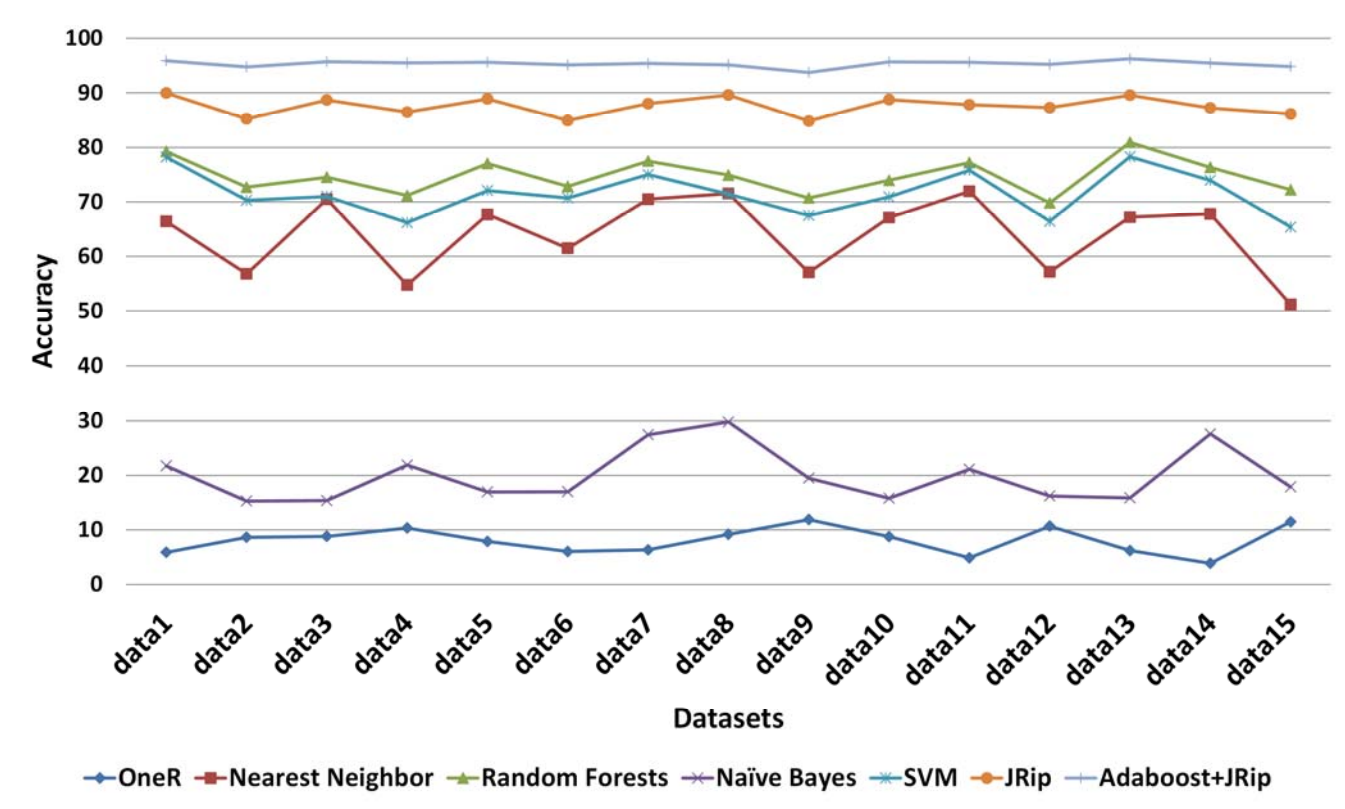
\includegraphics[width=\linewidth]{images/weka_accuracy2_cite.png}
        \caption{Original results \cite{borges_hink_machine_2014-1}}
    \end{subfigure}
    \caption{Accuracy for binary datasets}
    \label{fig:weka_acc2}
\end{figure}

\begin{figure}[H]
    \centering
    \begin{subfigure}[t]{0.5\textwidth}
        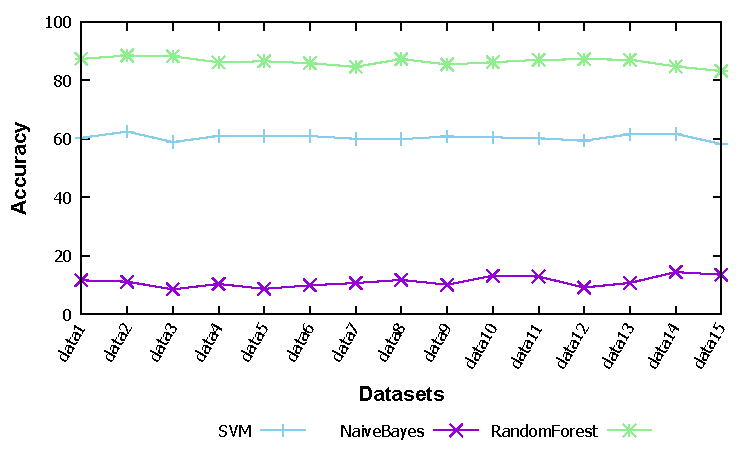
\includegraphics[width=\linewidth]{images/weka_accuracyall}
        \caption{Our attempt}
    \end{subfigure}%
    \begin{subfigure}[t]{0.5\textwidth}
        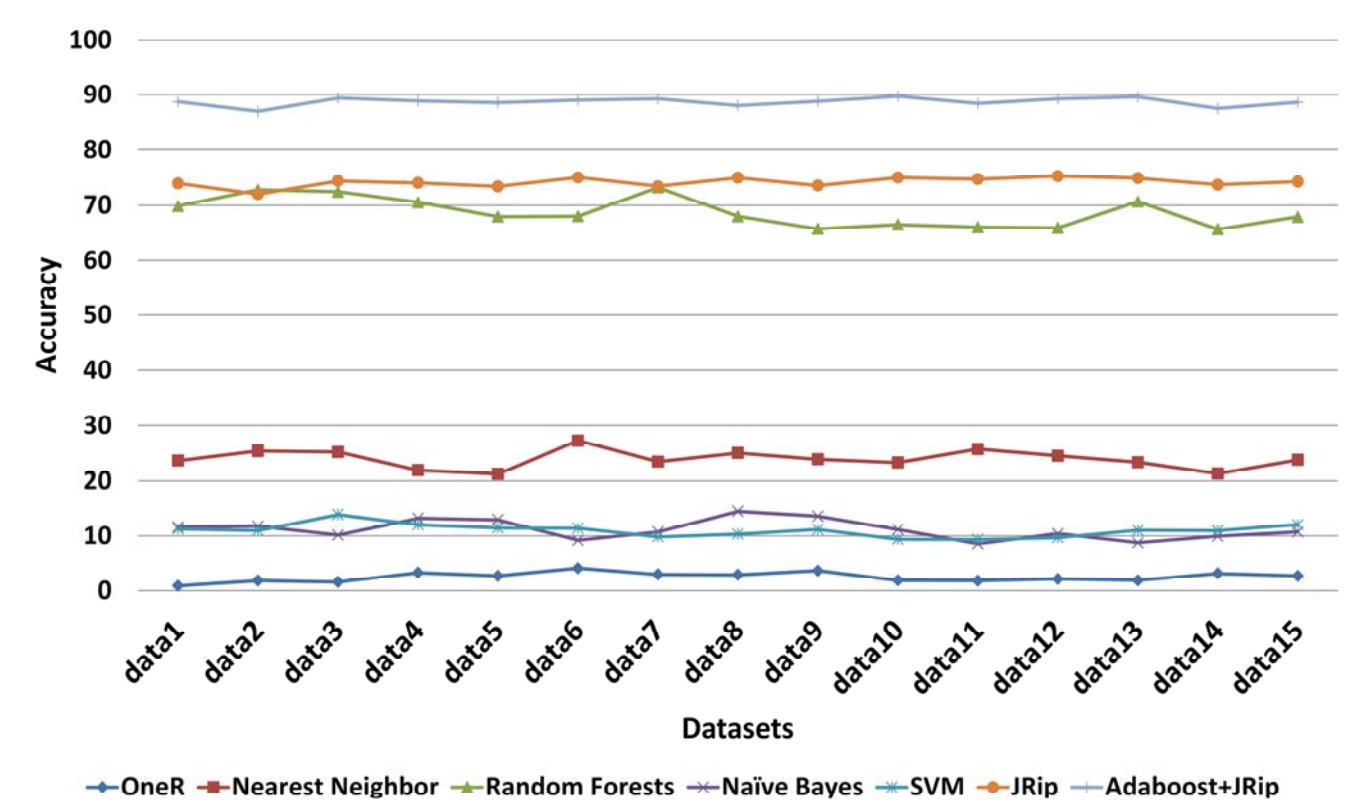
\includegraphics[width=\linewidth]{images/weka_accuracyall_cite.png}
        \caption{Original results \cite{borges_hink_machine_2014-1}}
    \end{subfigure}
    \caption{Accuracy for multiclass datasets}
    \label{fig:weka_accall}
\end{figure}

\begin{figure}[H]
    \centering
    \begin{subfigure}[t]{0.5\textwidth}
        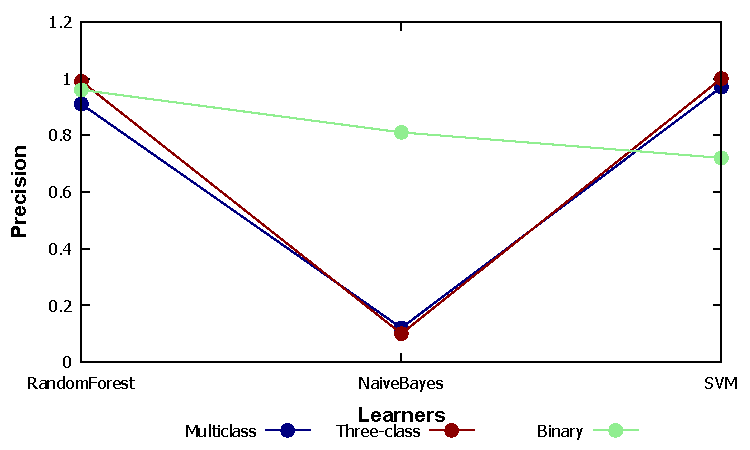
\includegraphics[width=\linewidth]{images/weka_precision}
        \caption{Our attempt}
    \end{subfigure}%
    \begin{subfigure}[t]{0.5\textwidth}
        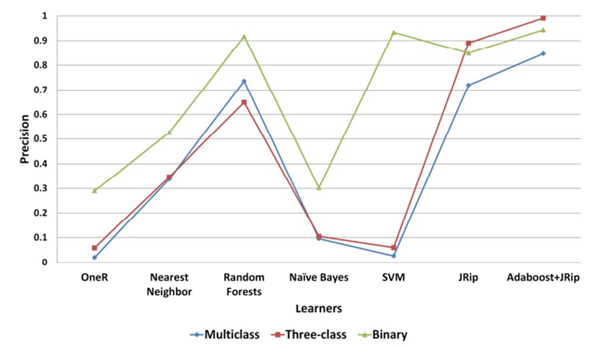
\includegraphics[width=\linewidth]{images/weka_precision_cite.png}
        \caption{Original results \cite{borges_hink_machine_2014-1}}
    \end{subfigure}
    \caption{Precision}
    \label{fig:weka_prec}
\end{figure}

\begin{figure}[H]
    \centering
    \begin{subfigure}[t]{0.5\textwidth}
        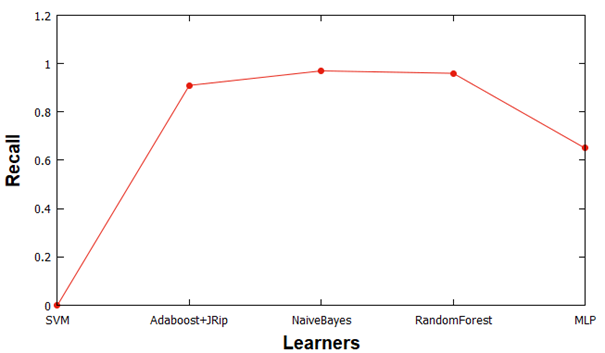
\includegraphics[width=\linewidth]{images/weka_recall}
        \caption{Our attempt}
    \end{subfigure}%
    \begin{subfigure}[t]{0.5\textwidth}
        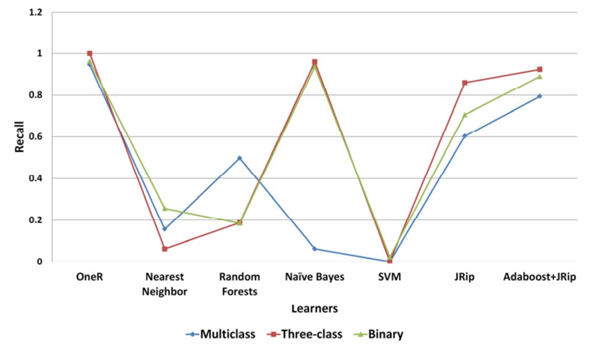
\includegraphics[width=\linewidth]{images/weka_recall_cite.png}
        \caption{Original results \cite{borges_hink_machine_2014-1}}
    \end{subfigure}
    \caption{Recall}
    \label{fig:weka_recall}
\end{figure}

\begin{figure}[H]
    \centering
    \begin{subfigure}[t]{0.5\textwidth}
        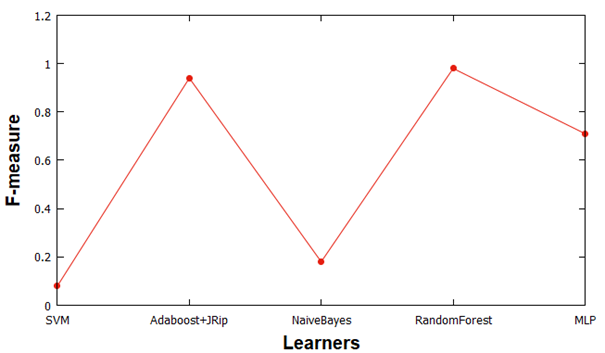
\includegraphics[width=\linewidth]{images/weka_f1}
        \caption{Our attempt}
    \end{subfigure}%
    \begin{subfigure}[t]{0.5\textwidth}
        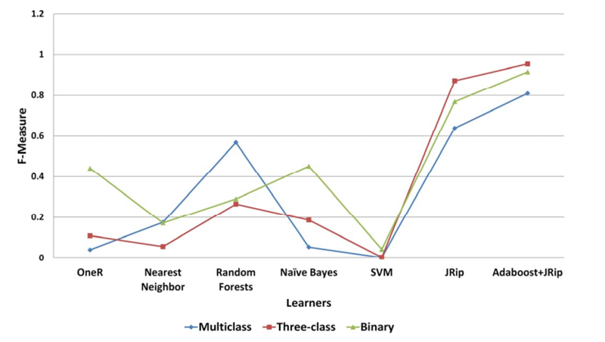
\includegraphics[width=\linewidth]{images/weka_f1_cite.png}
        \caption{Original results \cite{borges_hink_machine_2014-1}}
    \end{subfigure}
    \caption{F-measure}
    \label{fig:weka_f1}
\end{figure}

The obtained results indicate clearly that Random Forest algorithm is the more accurate and gives clearly the best results, with Adaboost+JRIP with slightly worse performance. On the other hand, the results presented in \cite{borges_hink_machine_2014-1} shows better results for Adaboost+JRIP. For SVM and Naïve Bayes the results are comparable, expect for precision value for SVM. The origin of this difference is so far unknown.

In addition to the mentioned algorithms, the multiplayer perceptron algorithm (MLP) was used in order to have an initial idea on its performance. The obtained results show that it is less accurate than Random Forest and Adaboost+JRIP algorithms with an accuracy of approximatively 90\%, the values of precision and recall are respectively 0.8 and 0.65, which are good results.

\section{scikit-learn} \label{sec:scikit_in_chap:methods}
The same approach described in previous section was made, but this time using scikit-learn Python3 library. The parameters for machine learning algorithms were chosen as follows:
\begin{itemize}
    \item RandomForest: number of trees in the forest = 100 and the maximum number of features when looking for a split is equal to $\log_2$ number of features,
    \item SVM: probability estimates enabled, maximum number of iterations = 1000, kernel size = 7000 MB,
    \item MLP: one hidden layer of 20 neurons, maximum number of iterations (instead of convergence) = 1000, stopping when validation score is not improving enabled,
    \item Naïve Bayes: default configuration.
\end{itemize}
Those parameters where chosen based on results of GridSearchCV class available in scikit-learn. It is used to compare different configurations of parameters in order to be able to chose the best one. The results will not be shown given the large amount of data obtained through this analysis, which is hard to present.

The results of classification analysis are shown on figure \ref{fig:scikit_results}. In contrast to Weka's result, precision, recall and f-measure indicators come with three different values:
\begin{itemize}
    \item micro: the metrics are determined globally by calculating true positives, false negatives and false positives,
    \item macro: the metrics are calculated for each class, then it gives their unweighted mean value,
    \item weighted: the metrics are calculated for each class, then it gives their weighted average value by the number of true instances for each class.
\end{itemize}

\begin{figure}[H]
\centering
\begin{subfigure}[t]{0.475\textwidth}
    \centering
    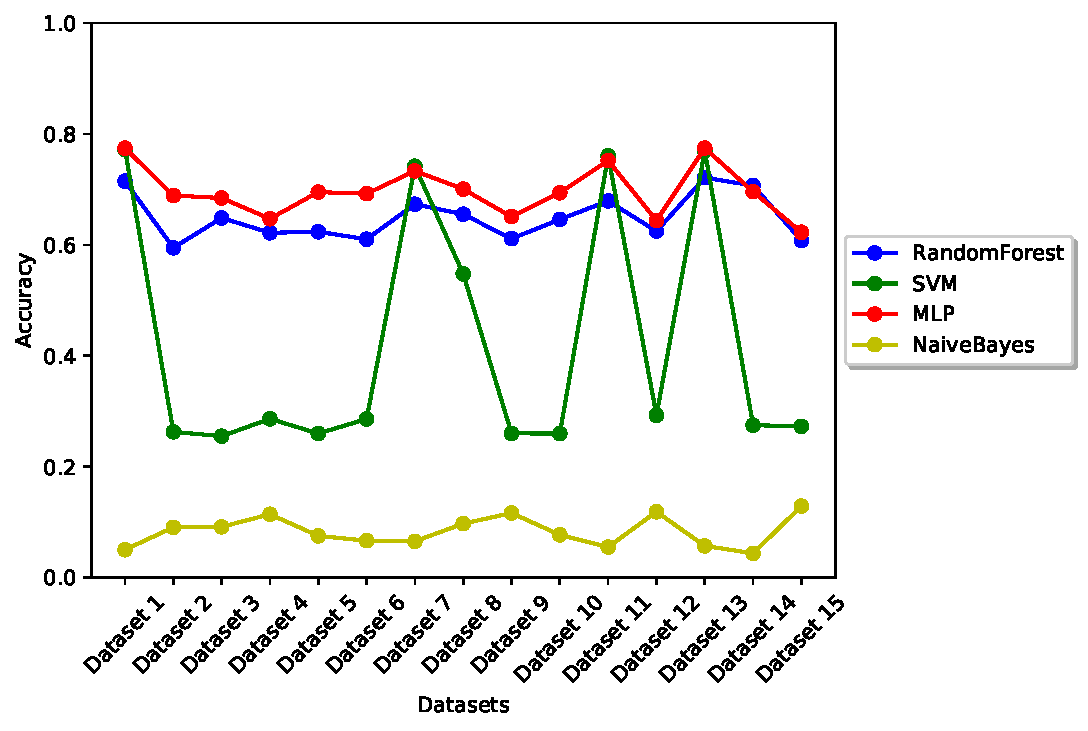
\includegraphics[page=1, width=\linewidth]{images/results_scikit.pdf}
    \caption{Accuracy}
    \label{fig:scikit_accuracy}
\end{subfigure}
\begin{subfigure}[t]{0.475\textwidth}
    \centering
    \includegraphics[page=3, width=\linewidth]{images/results_scikit.pdf}
    \caption{Precision}
    \label{fig:scikit_prec}
\end{subfigure}
\caption{scikit-learn results}
\end{figure}
\begin{figure}[H]\ContinuedFloat
\begin{subfigure}[t]{0.475\textwidth}
    \centering
    \includegraphics[page=4, width=\linewidth]{images/results_scikit.pdf}
    \caption{Recall\footnote{micro and weighted values are the same in this case.}}
    \label{fig:scikit_recall}
\end{subfigure}
\begin{subfigure}[t]{0.475\textwidth}
    \centering
    \includegraphics[page=2, width=\linewidth]{images/results_scikit.pdf}
    \caption{F-measure}
    \label{fig:scikit_f1}
\end{subfigure}
\caption{scikit-learn results}
\label{fig:scikit_results}
\end{figure}

It can be observed that the obtained results are partially different from those obtained using Weka. The results for MLP and Naïve Bayes are comparable to those from Weka, but on the other hand, the results for Random Forest and SVM differ considerably. This made MLP the most reliable classifier compared to others in this comparison.

It can be also deducted that Weka is calculating metrics globally (corresponds to micro in scikit-learn).

\section{scikit-learn further methods' analysis}

In addition to all that, scikit-learn enables the user to plot the receiver operating characteristic (ROC) curves for each class and the confusion matrix. The ROC curve represents the plot od true positive rate when the false positive rate changes. The confusion matrix on the other hand shows the normalized number (over the total number of samples) of predicted values of each class for each class. The results are illustrated on figures \ref{fig:ROCCM_RF}, \ref{fig:ROCCM_SVM}, \ref{fig:ROCCM_NB} and \ref{fig:ROCCM_MLP}.

\begin{figure}[H]
    \begin{subfigure}[t]{0.45\textwidth}
        \centering
        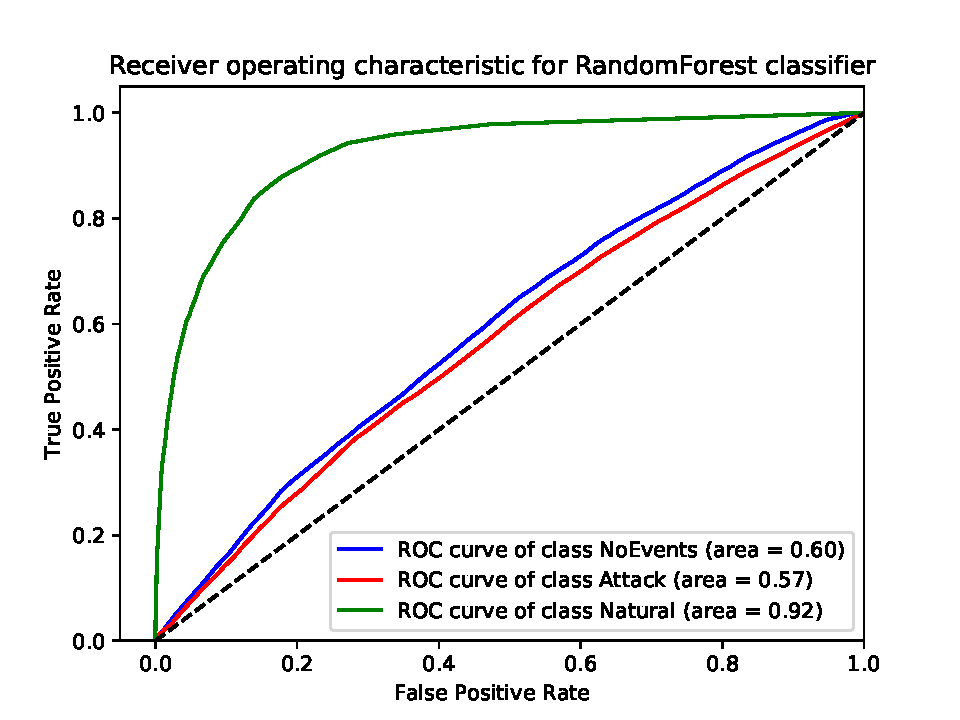
\includegraphics[page=1, width=\linewidth]{images/results_scikit/RandomForest}
        \caption{ROC Curve}
        \label{fig:scikit_RF_ROC}
    \end{subfigure}
    \begin{subfigure}[t]{0.45\textwidth}
        \centering
        \includegraphics[page=2, width=\linewidth, trim= 0 50 0 100, clip]{images/results_scikit/RandomForest}
        \caption{Confusion Matrix}
        \label{fig:scikit_RF_CM}
    \end{subfigure}
    \caption{Random Forest ROC curve and confusion matrix}
    \label{fig:ROCCM_RF}
\end{figure}

\begin{figure}[H]
    \begin{subfigure}[t]{0.45\textwidth}
        \centering
        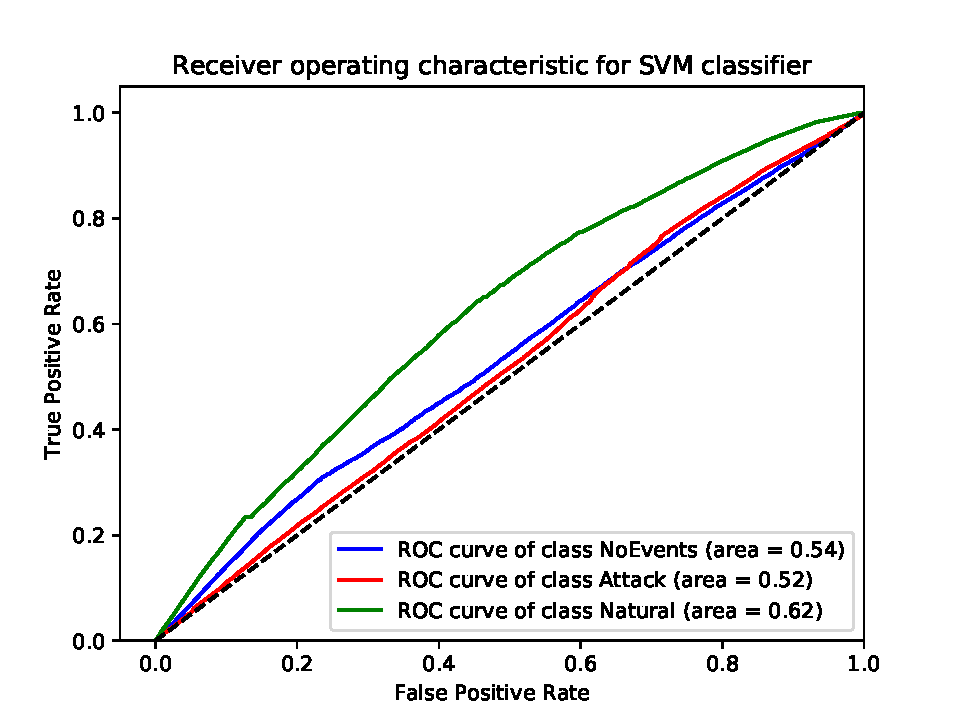
\includegraphics[page=1, width=\linewidth]{images/results_scikit/SVM}
        \caption{ROC Curve}
        \label{fig:scikit_SVM_ROC}
    \end{subfigure}
    \begin{subfigure}[t]{0.45\textwidth}
        \centering
        \includegraphics[page=2, width=\linewidth, trim= 0 50 0 100, clip]{images/results_scikit/SVM}
        \caption{Confusion Matrix}
        \label{fig:scikit_SVM_CM}
    \end{subfigure}
    \caption{SVM ROC curve and confusion matrix}
    \label{fig:ROCCM_SVM}
\end{figure}

\begin{figure}[H]
    \begin{subfigure}[t]{0.45\textwidth}
        \centering
        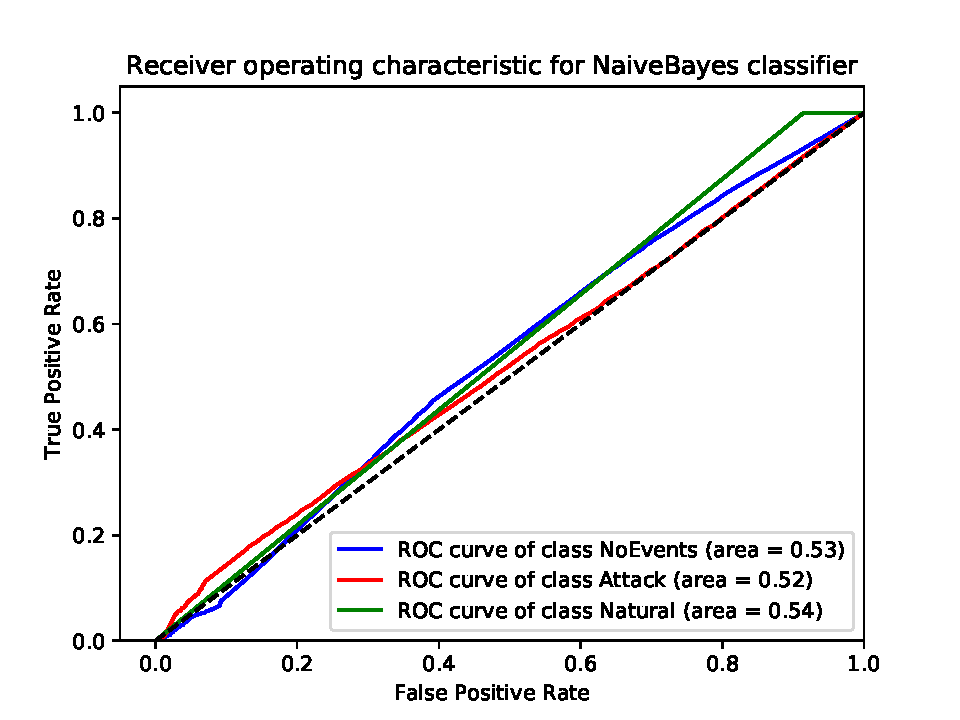
\includegraphics[page=1, width=\linewidth]{images/results_scikit/NaiveBayes}
        \caption{ROC Curve}
        \label{fig:scikit_NB_ROC}
    \end{subfigure}
    \begin{subfigure}[t]{0.45\textwidth}
        \centering
        \includegraphics[page=2, width=\linewidth, trim= 0 50 0 100, clip]{images/results_scikit/NaiveBayes}
        \caption{Confusion Matrix}
        \label{fig:scikit_NB_CM}
    \end{subfigure}
    \caption{Naïve Bayes ROC curve and confusion matrix}
    \label{fig:ROCCM_NB}
\end{figure}

\begin{figure}[H]
    \begin{subfigure}[t]{0.45\textwidth}
        \centering
        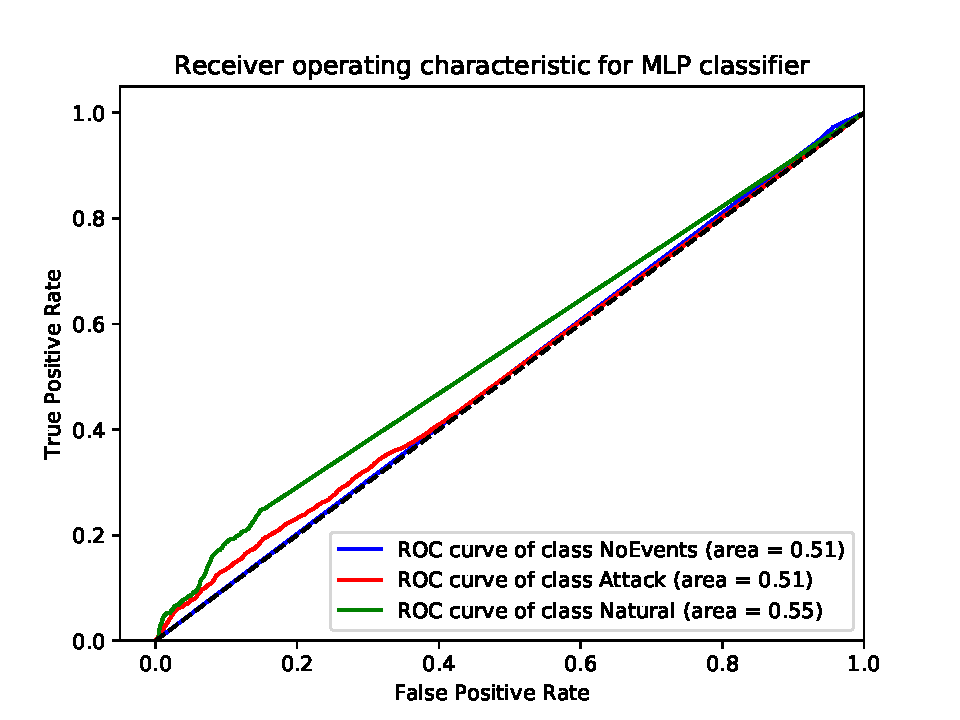
\includegraphics[page=1, width=\linewidth]{images/results_scikit/MLP}
        \caption{ROC Curve}
        \label{fig:scikit_MLP_ROC}
    \end{subfigure}
    \begin{subfigure}[t]{0.45\textwidth}
        \centering
        \includegraphics[page=2, width=\linewidth, trim= 0 50 0 100, clip]{images/results_scikit/MLP}
        \caption{Confusion Matrix}
        \label{fig:scikit_MLP_CM}
    \end{subfigure}
    \caption{MLP ROC curve and confusion matrix}
    \label{fig:ROCCM_MLP}
\end{figure}

The previous figures show that Random Forest classifier has the higher capacities to distinguish between the occurrence of each class, or it's absence. It's visible on both ROC curve and the confusion matrix, where the highest number of predictions is shown for the true positives for each class. SVM tends to predict only NoEvents and Attacks but does not really succeed in distinguishing between them. Naïve Bayes fails to make true predictions, it considers everything of class natural. Finally MLP, it succeeds in determining the class NoEvents, but does not distinguish over classes almost at all, despite the high accuracy (it is due because of the huge number of samples of class NoEvents).

Given this analysis, it can be deducted that Random Forest algorithm acts the best, and that is why it will be adapted in next chapters, in which, at first, an analysis of features and their importance will be made. However a deeper look at the amelioration of MLP will be also made later.

